\chapter{Comunicazione}
\vspace{15pt}

In questo capitolo sarà proposta una modellizzazione della trasmissione di informazione attraverso canali di comunicazione. 

\vspace{15pt}


\section{Trasmissione di informazione}
\label{sec:Trasmissione}
\vspace{10pt}


Il modello più semplice è costituito da una sorgente, un canale di comunicazione, ed un ricevente.\\
La sorgente sarà modellata da una variabile aleatoria $S$ a valori \va detti alfabeto sorgente e con \lep. Il fatto che la sorgente $S$ sia una variabile casuale va interpretato come l'incertezza su quale messaggio verrà inviato. In questo contesto un messaggio sarà formato da una serie di simboli presi da \va e posti uno di seguito all'altro.\\
Il ricevente sarà un'altra variabile casuale $R$ a valori \vb  detti alfabeto ricevente e con \leggeq, solitamente si avrà $m \geq n$.\\
Infine l'effetto di distorsione del canale sarà modellato dalla famiglia di probabilità condizionate \lepc  dove $p(j|i):= \mathbb{P}(R=b_j|S=a_i)$ (si noti che $p(j|i)$ corrisponde a $p_i(j)$ definito in \ref{sec:PropriEntropia}).\\
Un sistema di trasmissione ottimale avrà i due alfabeti di trasmissione e ricezione identici e nella distorsione avremo $p(i|i)$ il più vicino possibile ad 1, in questo modo quindi i valori ricevuti saranno quasi sicuramente gli stessi che sono stati inviati.\\
\begin{defi}
viene detta \textbf{mutua informazione}  tra $E$ ed $F$ il valore:
\begin{equation}
I(a_j,b_k)=- \log(q_k)+ \log(p(k|j))
\end{equation}
se $p_j=0$ allora diremo $I(a_j,b_k)=0$.\\
Dove E è l'evento $(S=a_j)$ che ha probabilità $p_j$, mentre $F$ è l'evento $(R=b_k)$ che avverrà con probabilità $q_k$.
\end{defi}
È importante notare che questa definizione di mutua informazione è diversa da quella data in \ref{defin:mutua} la quale si riferisce a due variabili casuali e non a due eventi come in questo caso.\\
Dato che $- \log(q_k)$ è l'informazione dell'evento $R=b_k$, mentre $- \log(p(k|j))$ è l'informazione aggiuntiva che ci darebbe la ricezione di $b_k$ sapendo già per certo che è stato spedito $a_j$, possiamo interpretare $I(a_j,b_k)$ come la quantità di informazione su $R=b_k$ che ci è data dall'evento $S=a_j$. In altre parole è la quantità di informazione che è spedita attraverso il canale.
\begin{teo} \label{teo:7.1}
Per ogni $1\leq j \leq n , 1 \leq k, \leq m$ si ha:
\begin{enumerate}
\item $I(a_j,b_k)=- \log(\frac{p_{jk}}{p_j q_k})$
\item $I(a_j,b_k)=- \log(p_j)+ \log(q(j|k))$
\item $I(a_j,b_k)=I(b_k,a_j)$
\item se gli eventi $S=a_j$ e $R=b_k$ sono indipendenti allora $I(a_j,b_k)=0$
\item $I(S,R)=\sumj \sumk p_{jk}I(a_j,b_k)$.
\end{enumerate}
\end{teo}
\begin{proof}
\begin{enumerate}
\item deriva banalmente da $p(k|j)=\frac{p_{jk}}{q_k}$
\item si ricava sostituendo in 1. $q(j|k)=\frac{p_{ik}}{q_k}$
\item deriva da 2.
\item ricordando che nel caso siano indipendenti $p_{jk}=p_jq_k$ si ricava immediatamente da da 1.
\item si ricava da 1. e dal primo punto del teorema \ref{teo:6.7}
\end{enumerate}
\end{proof}
Il punto 3. del sistema ci mostra la curiosa caratteristica per cui se in un sistema si invertono sorgente e ricevente abbiamo che l'informazione su $a_j$ contenuta in $b_k$ è la stessa di quella contenuta in $a_j$ su $b_k$ quando il canale funziona normalmente. Si può dimostrare che $I(S,R)\geq 0$ sempre.


Supponiamo ora di scegliere un canale e di fissare \lepc . Vogliamo ora fare in modo che il canale trasmetta più informazione possibile, per fare ciò le uniche variabili del sistema rimaste ancora libere con cuoi possiamo lavorare sono $\{p_1...p_n \}$ .
\begin{defi}
viene definita \textbf{capacità del canale C} la quantità:
\begin{equation}
C:= \max_{ \{ p_1...p_n \}} I(S,R)
\end{equation}
dove il massimo è scelto tra tutte le possibili leggi di probabilità della variabile $S$
\end{defi}
Operativamente spesso è preferibile vedere la capacità del canale C come:
\begin{equation}
C=max(H(R)-H_S(R))
\end{equation}
ottenuta utilizzando la definizione di mutua informazione tra variabili casuali \ref{defin:mutua}.\\
\begin{oss} \label{oss:bsc}
Il più semplice esempio di canale di comunicazione che possiamo trovare è un canale binario simmetrico, esso avrà grande rilevanza in seguito. È formato da una sorgente  con alfabeto $\{ 0 , 1 \}$ e come specificato nella figura il \textit{rumore} del canale è definito attraverso un parametro $p$
\\


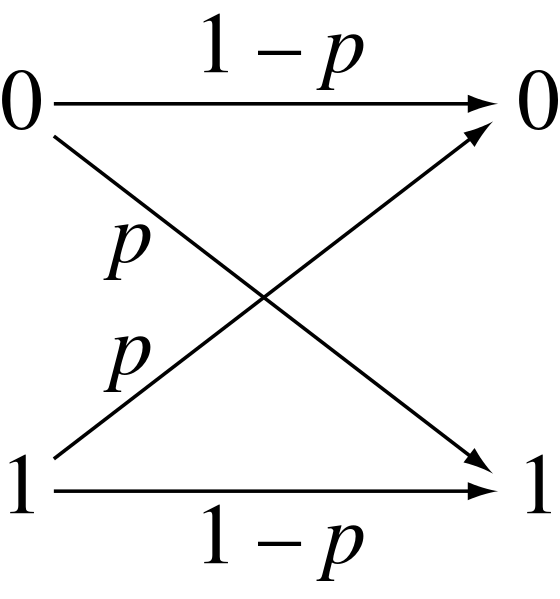
\includegraphics[scale=0.20]{Binary_symmetric_channel.png} \label{fig:bsc}
%\begin{tikzpicture}
%\draw[thick,->] (0,0) -- (6,-3) node[anchor=south east] {$\epsilon$}; 
%\draw[thick,->] (0,-3) -- (6,0) node[anchor=south east] {$\epsilon$}; 
%\end{tikzpicture}
\\

Supponiamo che la sorgente trasmetta $1$ con probabilità $\epsilon$ e $0$ con probabilità $(1- \epsilon)$, $S$ quindi sarà una variabile casuale con distribuzione di Bernoulli a parametro $\epsilon$. Ovviamente anche la ricevente $R$ sarà una variabile casuale di Bernoulli, chiamiamo $q=\mathbb{P}(Y=1)$ il suo parametro e andiamo a calcolarne il valore:
\[
\begin{split}
q & =\mathbb{P}(Y=1)\\
&=\mathbb{P}(Y=1|X=0)\mathbb{P}(X=0)+\mathbb{P}(Y=1|X=1)\mathbb{P}(X=1)\\
&=p (1-\epsilon) + (1-p)\epsilon\\
&= p + \epsilon -2p\epsilon
\end{split}
\]
Per comodità denotiamo gli eventi
$$a_0:=(S=0),\ \ a_1:=(S=1),\ \ b_0:=(R=0),\  \ b_1:=(R=1)$$
Calcoliamo $I(a_1,b_1),I(a_0,b_0),I(a_0,b_1),I(a_1,b_0)$.\\
Dal teorema \ref{teo:7.1} abbiamo:
\[
\begin{split}
I(a_1,b_1)& = I(b_1,a_1) \\
&=-\log(q)+\log(1-p)\\
&=\log \bigg( \frac{1-p}{q} \bigg)
\end{split}
\]
analogamente otteniamo
\[
\begin{split}
& I(a_0,b_1)=\log \bigg( \frac{p}{q} \bigg)\\
& I(a_0,b_0)=\log \bigg( \frac{1-p}{1-q} \bigg)\\
& I(a_1,b_0)=\log \bigg( \frac{p}{1-q} \bigg)
\end{split}
\]
Per quanto riguarda la capacità si ha:
$$C=\max(H(R)-H_S(R))$$
dove:
\[
\begin{split}
&H(R)=-q \log(q)-(1-q)\log(1-q) \\
& \begin{split}
H_S(R) & = - p_{00} \log(p(0|0)) - p_{01} \log(p(1|0)) -p_{10} \log(p(0|1)) -p_{11} \log(p(1|1)) \\
& = -(1-\epsilon)(1-p) \log (1-p)- (1- \epsilon)p \log (p)- \epsilon (1-p)\log(1-p)- \epsilon p \log (p)\\
&= - (1-p) \log (1-p)- p log(p)
\end{split}
\end{split}
\]
Dato che il massimo va scelto tra tutte le possibili distribuzioni di $S$ abbiamo quindi che $\epsilon$ è il parametro che possiamo far variare, notiamo che $H_S(R)$ non dipende da $\epsilon$ e quindi sarà una \textit{costante}. Per quanto riguarda $H(R)$ essa dipenderà da $\epsilon$ attraverso $q$, e quindi ricordando che $H(X)\leq log(n)$ scegliendo $\epsilon= \frac{1}{2}$ otteniamo $1=H(R)=\log(2)$. Riassumendo
$$C=\max(H(R)-H_S(R))=1-H_S(R)$$
Possiamo notare che $C$ sarà una funzione di $p$ ed avrà minimo quando $p=\frac{1}{2}$ e massimo agli estremi ($p=0$ o $p=1$).
Può sembrare che la quantità d'informazione inviata attraverso un canale non possa essere scelta arbitrariamente vicina alla capacità $C$ del canale, ma che sia dettata dalla distribuzione di $S$. Vedremo nel prossimo capitolo come, grazie all'introduzione di nuovi oggetti sarà possibile modificare a nostro favore la distribuzione dei dati inviati
\end{oss}
\vspace{15pt}


\section{Codici}
\label{sec:Codici}
\vspace{10pt}

In questo paragrafo daremo un idea di ciò che si intende con \textit{codice} nella matematica per poi applicarci la nostra conoscenza sulla trasmissione di informazione.\\
\begin{defi}
L'\textbf{alfabeto di un codice, C} è un insieme \acode i cui elementi $c_i$ sono chiamati \textbf{simboli}.\\
Una \textbf{parola-codice} o \textbf{parola del codice} è una serie di simboli $c_{i_1}...c_{i_n}$.\\
Il numero $n$ sarà la \textbf{lunghezza} della parola-codice.\\
Un \textbf{messaggio} sarà una successione di parole-codice.
\end{defi}
Il processo di codifica di un messaggio è quello di mappare ogni singolo  simbolo dell'alfabeto di un linguaggio con una parola-codice.\\
Un esempio di codice che poi utilizzeremo lungo tutto il capitolo è dato dal codice binario:
$$C=\{0, 1 \}$$
Il nostro obiettivo sarà capire cosa succede all'informazione trasmessa modificando il percorso del messaggio nel modo seguente:
$$ SORGENTE \to codificatore \to CANALE \to decodificatore \to RICEVENTE$$
\\
Per fare cioè ci serviremo di un'importantissima classe di codici: quella dei \textit{codici istantanei o codici prefisso}.
\begin{defi}
Sia $c_{i_1}...c_{i_n}$ una parola del codice. Preso $k<n$ se  $c_{i_1}...c_{i_k}$
è anch'essa una parola tale parola si dirà \textbf{prefisso}.\\
Un codice in cui non esistono parole che sono prefisso di altre è detto \textbf{codice istantaneo} o \textbf{codice prefisso}.
\end{defi}.
\begin{lem}
Ogni codice istantaneo è decodificabile in modo univoco, inoltre per avere una codifica univoca non è necessario aspettare di ricevere tutto il messaggio.
\end{lem}

Viste le forti proprietà dei codici istantanei è naturale chiedersi quando sia possibile creare codici con queste caratteristiche.

\begin{teo} \label{teo:disugKM} (\textit{Disugiaglianza di Kraft-McMillan})\\
Dato un alfabeto sorgente composto da $n$ simboli che deve essere codificato allora esiste un codice istantaneo con alfabeto di $r$ simboli e parole di lunghezza $l_i \ (1 \leq i \leq n)$ se e solo se 
\begin{equation} \label{eq:disugKM}
\sumin r^{-l_i}\leq 1.
\end{equation} 
\end{teo}

La disuguaglianza di \textit{Disugiaglianza di Kraft-McMillan} ci garantisce l'esistenza di codici che soddisfano le nostre richieste e, attraverso \ref{eq:disugKM} , ci aiuta a trovare tali codici. Il passo successivo sarà chiederci come si può scegliere il migliore tra tutti i codici istantanei. Cominciamo con una definizione

\begin{defi}
Dato un alfabeto sorgente $S$ \va  con \lep  a cui viene associato un codice istantaneo posiamo considerare una variabile casuale $L$ con immagine $\{ l_1...l_n \}$ (dove $l_i$ corrisponderà al numero di simboli necessari per scrivere in codice il simbolo $a_i$) e \lep  la stessa di $S$. Preso il valore di aspettazione di $L$:
$$\mathbb{E}(L)=\sumin p_j l_j$$ 
diremo che \textbf{il codice è ottimale} se minimizza $\mathbb{E}(L)$.
\end{defi}
È chiaro che in generale un codice ottimale non è unico infatti dato un qualsiasi codice ottimale che utilizzi un alfabeto di almeno due lettere ci basterà considerare un codice in cui le lettere vengono permutate per ottenere un nuovo codice ottimale.\\
Enunciamo ora un sorprendente teorema che ci permette di mettere in relazione il valore di aspettazione di $L$ con l'entropia dell'alfabeto sorgente, dandoci quindi utili informazioni sul valore di aspettazione di un codice ottimale.
 
\begin{teo}(\textit{Teorema della codifica di sorgente per simboli di codice})\\
Dato un alfabeto sorgente $S$ con \lep vale:
\begin{enumerate}
\item Per ogni codice istantaneo con una alfabeto di $r$ simboli abbiamo che
\begin{equation}
\frac{H(S)}{\log (r)} \leq \mathbb{E}(L)
\end{equation}
con l'uguaglianza se e solo se $p_j=r^{l_j}$ $(1 \leq j \leq n)$
\item esiste un codice istantaneo formato da $r$ simboli per cui
\begin{equation}
\frac{H(S)}{\log (r)} \leq \mathbb{E}(L) < \frac{H(S)}{\log (r)} +1
\end{equation}
\end{enumerate}
\end{teo}

\begin{proof}
\item Definiamo $\{q_1...q_n \}$ con
\begin{equation}
q_j=\frac{r^{-l_j}}{\sumi r^{-l_i}}
\end{equation}
abbiamo che l'insieme dei $q_i$ forma una distribuzione di probabilità infatti:
\[
\begin{split}
\sumj q_j& = \sumj \frac{r^{-l_j}}{\sumi r^{-l_i}}\\
&= \frac{\sumj  r^{-l_j}}{\sumi r^{-l_i}} =1
\end{split}
\]

e ovviamente $q_j\geq 0$.\\
Possiamo quindi utilizzare la disuguaglianza di Gibbs nel caso discreto: $- \sumin p_i \log(p_i) \leq - \sumin p_i \log(q_i)$ per $\{p_1...p_n \}$ e $\{q_1...q_n \}$ distribuzioni di probabilità (deriva immediatamente dal caso continuo \ref{teo:GibbsContinuo}) ottenendo:
\[
\begin{split}
H(S)& = - \sumj p_j \log(p_j) \\
& \leq  - \sumj p_j \log(q_j)\\
& =  - \sumj p_j \log \bigg(\frac{r^{-l_j}}{\sumi r^{-l_i}} \bigg)\\
& =  - \sumj p_j \log ( r^{-l_j}) +\sumj p_j \log \bigg( \sumi r^{-l_i} \bigg)\\
& \leq - \sumj p_j \log ( r^{-l_j}) +\sumj p_j \log (1)\\
& =\sumj p_j l_j \log ( r)\\
&= \mathbb{E}(L)\log (r)
\end{split}
\]
dove per ottenere la quinta riga abbiamo utilizzato la disugiaglianza di Kraft-McMillan \ref{teo:disugKM}.\\
Dalle condizioni delle disuguaglianze di Gibbs e Kraft abbiamo che si ha l'uguaglianza se e solo se $p_j=r^{-l_j}$
\item  Il primo punto dimostra anche il primo membro della disuguaglianza, mostriamo ora la validità della seconda parte.\\
Imponiamo $l_j =  -\lceil \log_r(p_j) \rceil$ cioè  $- \log_r(p_j) \leq l_j < - \log_r(p_j) +1$ e quindi 
$$r^{-l_j} \leq p_j \implies $$ 
$$  \sumj r^{-l_j} \leq \sumj p_j=1.$$
Quindi per la disuguaglianza di Kraft esiste un codice di tale lunghezza con variabile casuale associata $L$. Abbiamo:
\[
\begin{split}
H(L)& =  \sumj p_j l_j \\
& <   - \sumj p_j  \log_r(p_j) +1\\
& = - \sumj p_j  \frac{\log(p_j)}{\log(r)} +1 \\
& =  \frac{H(S)}{ \log (r)} +1
\end{split}
\]
\end{proof}
Il teorema appena dimostrato è detto primo teorema di Shannon e fu dimostrato proprio dal matematico Americano nel 1948.\\

\vspace{15pt}


\section{Regole di decisione}
\vspace{10pt}

Mettiamoci nella situazione
$$ SORGENTE \to codificatore \to CANALE \to decodificatore \to RICEVENTE$$
e concentriamoci sul segmento $codificatore \to CANALE \to decodificatore$.\\
Supponiamo che $C:=\{ x_1 ..x_n \}$ sia l'insieme di tutte le possibili parole del codice che possono essere trasmesse dal canale e che $y$ sia la parola ricevuta. Per decidere quale parola $x_i$ è stata trasmessa possiamo utilizzare il \textit{principio di massima verosimiglianza}:\\
Date le probabilità condizionate $p(y|x_i):=(R=y|S=x_i)$ decideremo che la parola inviata è $x_k$ se
\begin{equation} \label{eq6}
p(y|x_k )\geq p(y|x_i) \ \forall i\neq k
\end{equation}
Nel caso in cui più $x_s$ soddisfino \ref{eq6} $x_k$ verrà scelta in modo casuale tra le varie $x_s$.\\
Ovviamente la nostra scelta di $x_k$ non ci garantisce che sia stata effettivamente inviata $x_k$.\\
Esistono altri principi sui quali basarsi per la scelta di $x_k$ nel caso di codici binari ad esempio si può definire \textit{distanza di Hammning} per aiutarsi nella decisione:
\begin{defi}
date due parole di un codice binario $a,b$ si definisce \textbf{distanza di Hamming} il numero di simboli per cui $a$ è differente da $b$
\end{defi}
Utilizzando questa distanza è naturale scegliere come parola $x_k$ inviata quella che dista meno dalla parola ricevuta $y$.

\begin{teo}
Per un canale binario simmetrico come quello visto in \textbf{Osservazione} \ref{oss:bsc} dove $0 \leq p < \frac{1}{2}$, fissata una parola $y$ l'insieme $\{ x_s \}$ delle parole con distanza di Hamming minima da $y$ coincide con quello delle parole a verosimiglianza massima rispetto a $y$
\end{teo}
\begin{proof}
Sia $m$ la lunghezza di $y$, la probabilità che sia stata inviata una parola $x$ tale che $d(x,y)=\epsilon \leq m$ è:
$$\mathbb{P}(Y=y|X=x)= p^{\epsilon}(1-p)^{m-\epsilon}=(1-p)^m \bigg( \frac{p}{1-p} \bigg)^{\epsilon}$$
Dato che $0 \leq p < \frac{1}{2} \implies \frac{p}{1-p}<1 $ e quindi $\mathbb{P}(Y=y|X=x)$ ha massimo quando $\epsilon$ è minimo.
\end{proof}
Come già accennato in precedenza, la scelta della parola inviata $x$ non è mai certa e si possono commettere errori, in particolare detto $E$ l'evento \textit{"viene commesso un errore"} chiamiamo $\mathbb{P}(E|S=x_j)$ la probabilità che venga commesso un errore sapendo che è stato inviato $x_j$.
\begin{defi}
La \textbf{probabilità media di errore} è naturalmente definita come:
$$P(E)=\sum_{j=1}^{N}\mathbb{P}(E|x_j)\mathbb{P}(S=x_j)$$
\end{defi}
Osserviamo che $\mathbb{P}(E|x_j)$ e di conseguenza anche $P(E)$ dipenderanno dal tipo di regola che adotteremo per ipotizzare chi la parola inviata.\\
Per semplicità d'ora in avanti utilizzeremo una distribuzione uniforme sull'insieme $C$ delle parole del codice cioè $\mathbb{P}(S=x_j)=\frac{1}{n}$.\\
Un'importante regola di decisione utilizzata nei canali binari simmetrici si basa sul fatto che, supponendo di aver ricevuto la parola $y$, la probabilità di aver commesso un errore al $j-esimo$ posto è una variabile casuale $X_j$ di Bernoulli con parametro $p$ e quindi il numero di errori totali commessi in $y$ sarà la somma di $d$ variabili di Bernoulli cioè una variabile casuale $S(d,p)$ con distribuzione binomiale e parametri $d,p$ la cui media è
$$\mathbb{E}[S(d,p)]=dp$$.\\
Per enunciare la nostra regola di decisione pensiamo le parole del codice inviate e ricevute come vettori di dimensione $d$, si consideri poi una palla $d-dimensionale$ $\mathcal{B}_d(y,d(p+v)$ con $v$ numero arbitrario piccolo a piacere. 
\begin{defi} \label{defi:decisione}
Ricevuta $y$ diremo che la parola che è stata inviata è $x$ solo se $x$ è l'unica parola all'interno della palla, diremo che è stato commesso un errore se nella palla non sono presenti parole oppure ce ne sono due o più.
\end{defi}
In particolare questa regola nel caso in cui $S(d,p)>d(p+v)$ dichiarerà che è stato commesso un errore

\vspace{15pt}


\section{Teorema di Shannon}
\vspace{10pt}

È chiaro che per noi l'aspetto più importante di un canale comunicativo è la quantità di informazione media che viene effettivamente trasmessa dal canale. Per rendere in modo matematico questo concetto ricordiamo che il nostro canale di comunicazione altro non è che due variabili casuali $S,R$ legate da una legge di probabilità condizionata e come si è visto nella sezione \ref{sec:PropriEntropia} l'informazione scambiata tra queste due variabili è data dalle definizione \ref{defin:mutua}. Riscriviamo quanto detto.
\begin{defi}
Si dice \textbf{velocità di trasmissione}, $V$ la quantità media di informazione contenuta in un simbolo dell'alfabeto sorgente che riesce ad essere trasmessa da un canale in cui vengono trasmessi simboli ala velocità di uno al secondo
$$V:=H(R)-H_S(R)$$
\end{defi}
Prendiamo ad esempio il nostro solito canale binario abbiamo quindi che, se sono stati emessi $n$ simboli, allora i \textit{bit} di informazione trasmessi saranno $[2^{nV}]$ dove con le parentesi quadre intendiamo approssimare per eccesso all'intero più vicino.\\
Notiamo che indicata con $H_b(p)$ l'entropia di una variabile casuale di Bernouli di parametro p abbiamo che $H_b(p)=-p \log(p)- (1-p) \log(1-p) =H(R|S)$ dove $S$ è una variabile casuale di Bernoulli con parametro $\epsilon$ e con un errore del canale pari a $p$.\\
Prima di vedere il teorema di Shannon prepariamo il terreno dimostrando un lemma tecnico utile poi per la dimostrazione del teorema.
\begin{lem}
Sia $0 \leq p < \frac{1}{2}$ e $m\in \mathbb{N}$ allora vale
\begin{equation} \label{eq:7.6}
\sume \leq 2^{mH_b(p)}
\end{equation}
\end{lem}
\begin{proof}
 \[
\begin{split}
1&=(p+(1-p))^m \\
& = \sum_{k=0}^{[m]}  {m \choose k} p^k (1-p)^{m-k}\\
& \geq   \sume p^k (1-p)^{m-k} \\
&=(1-p)^m \sume \bigg( \frac{p}{1-p} \bigg)^k
\end{split}
\]
Dato che $0 \leq p < \frac{1}{2}$ allora anche $\bigg( \frac{p}{1-p} \bigg)<1$ e quindi
$$\bigg( \frac{p}{1-p} \bigg)^k \geq \bigg( \frac{p}{1-p} \bigg)^{mp} \ \ \forall 0\leq k \leq [mp]$$
riprendendo da sopra abbiamo:
$$1 \geq (1-p)^m  \bigg( \frac{p}{1-p} \bigg)^{mp} \sume$$
da cui riordinando la disequazione:
$$\sume \leq [p^{-p}(1-p)^{-(1-p)}]^m= 2^{mH_b(p)}$$
dove l'ultima uguaglianza si ha ricordando che in generale vale $2^{-H(X)}=p_1^{p_1}...p_n^{p_n}$
\end{proof}
Rifacendoci a \ref{defi:decisione} definiamo $A$ come l'evento in cui non ci sono parole del codice all'interno della palla, $B$ l'evento in cui ve ne sono più di una infine $E$ quello in cui è stato commesso un errore. Chiaramente $E=A\cup B$ ed inoltre 
\begin{equation}\label{eq:7.7}
\mathbb{P}(E)=\mathbb{P}(A)+ \mathbb{P}(B)
\end{equation}
essendo $\mathbb{P}(A \cap B)=0$.\\
Premettiamo al teorema due lemmi che ne renderanno immediata la dimostrazione.

\begin{lem}
Per ogni fissato $\delta_1>0$, scelto $d$ sufficientemente grande vale:
$$\mathbb{P}(A)\leq \delta_1$$   
\end{lem}
\begin{proof}
Ricordando cos'è l'evento $A$ troviamo che 	
 \[
\begin{split}
\mathbb{P}(A)&=\mathbb{P}(S(d,p)>d(p+v))\\
& = \mathbb{P}(S(d,p)-dp>dv)\\
& \leq \mathbb{P}(|S(d,p)-dp|>dv)
\end{split}
\]
Ricodrando che $S(d,p)$ è una variabile casuale con distribuzione binomiale a parametri $d,p$
Ora applicando la disuguaglianza di Chebyshev otteniamo:
$$\mathbb{P}(A)\leq \frac{p(1-p)}{dv}$$
che conclude la nostra dimostrazione
\end{proof}

\begin{lem}
Siano $\rho$ e $\delta_2$ due numeri reali non negativi e supponiamo che le parole del codice siano $M=2^{d(C-\rho)}$ dove $C=1-H_b(p)$ è la capacità del canale allora, per $d$ sufficientemente grande vale:
$$\mathbb{P}(B)\leq \delta_2$$
\end{lem}
\begin{proof}
Supponiamo che nella palla $\mathcal{B}(y,r)$ (dove $r=d(p+v)$) ci siano due o più parole. Sia $x_i$ quella con \textit{distanza di Hamming} da y minore. Abbiamo che
\[
\begin{split}
\mathbb{P}(B)&=\mathbb{P}\bigg( (x_i\in \sig) \cap \bigg( \bigcup_{j=1,j\neq i}^M (x_j \in \sig ) \bigg) \bigg)\\
&\leq \mathbb{P}\bigg( \bigcup_{j=1,j\neq i}^M (x_j \in \sig ) \bigg)\\
& \leq \sum_{j=1,j\neq i}^M \mathbb{P}(x_j\in \sig)\\
&= (M-1) \mathbb{P}(x_j \in \sig ) \textit{per alcuni } \ 1\leq j \leq M
\end{split}
\]
Dove per arrivare all'ultima riga abbiamo tenuto conto del fatto che per ipotesi $x_j$ sono identicamente distribuite.
Troviamo ora $\mathbb{P}(x_j\in \sig)$. Abbiamo che $x_j$ appartiene a $\sig$ solo se ha almeno $[r]$ errori e ricordando che la probabilità di avere esattamente $k$ errori è: $\frac{1}{2^d} {d \choose k}$ abbiamo che:
$$\mathbb{P}(x_j\in \sig)=\frac{1}{2^d} \sum_{k=0}^{[r]} {d \choose k}\leq \frac{2^{dH_b(p+v)}}{2^d}=2^{-d(1-H_b(p+v))}$$
quindi unendo questi due ultimi risultati otteniamo:
\[
\begin{split}
\mathbb{P}(B) &\leq (M-1)2^{-d(1-H_b(p+v))}\\
&\leq M2^{-d(1-H_b(p+v))}\\
& = 2^{d(C-\rho)}2^{-d(1-H_b(p+v))}\\
& = 2^{d(-H_b(p)-\rho}2^{-d(1-H_b(p+v))}\\
& =2^{d(H_b(p+v)-H_b(p)-\rho)}
\end{split}
\]
Dato che $H_b(x)$ è una funzione continua crescente per $x< \frac{1}{2} $ possiamo trovare $v$ abbastanza piccolo tale che $H_b(p+v)-H_b(p)<\rho$ in modo che 
$$(H_b(p+v)-H_b(p))-\rho < 0$$
e quindi prendendo $d$ sufficientemente grande possiamo fare in modo che $2^{d((H_b(p+v)-H_b(p))-\rho )}<\delta_2$ permettendoci di concludere.
\end{proof}


\begin{teo} (\textit{Teorema Fondamentale di Shannon})
Dati $\delta , \rho > 0$ possiamo trovare un codice tale per cui se la velocità di trasmissione in un canale binario simmetrico è $V=C-\rho$ allora
$$\mathbb{P}(E)< \delta$$
\end{teo}
\begin{proof}
Ricordando che $E=A\cup B$, il risultato discende direttamente dai due lemmi precedenti
\end{proof}
Seguendo una dimostrazione analoga il teorema è dimostrabile per ogni canale.




